\documentclass[12pt]{article}
\usepackage{graphicx}
\usepackage{geometry}
\usepackage{setspace}
\usepackage{titlesec}
\usepackage{tocloft}
\usepackage{fancyhdr}
\usepackage{hyperref}
\usepackage{xcolor}
\usepackage[T1]{fontenc}
\usepackage[utf8]{inputenc}
\usepackage[ngerman]{babel}

\geometry{a4paper, margin=2.5cm}
\setstretch{1.5}
\titleformat{\section}[block]{\LARGE\bfseries\color{black}}{}{0em}{\filcenter}
\titlespacing*{\section}{0pt}{3.5ex plus 1ex minus .2ex}{2.3ex plus .2ex}
\renewcommand{\cftsecleader}{\cftdotfill{\cftdotsep}}
\renewcommand{\contentsname}{Inhaltsverzeichnis}
\renewcommand{\cftaftertoctitle}{\par\nobreak\bigskip\bigskip\bigskip}
\setlength{\cftbeforesecskip}{0.5em}
\setlength{\cftaftertoctitleskip}{2cm}
\hypersetup{
    colorlinks=true,
    linkcolor=blue,
    filecolor=magenta,
    urlcolor=cyan,
}

\pagestyle{fancy}
\fancyhf{}
\fancyhead[R]{\thepage}
\fancyhead[L]{\nouppercase{\leftmark}}
\renewcommand{\headrulewidth}{0pt}
\fancyfoot[C]{\thepage}
\renewcommand{\footrulewidth}{0pt}

\definecolor{lightgray}{RGB}{240,240,240}

\begin{document}

\begin{titlepage}
    \centering
    \vspace*{3cm}
    {\Huge\bfseries\textcolor{blue}{\MakeUppercase{ Die Magische Universität: Ein Jahr im Verborgenen }}\par}
    \vspace{0.5cm}
    {\Large\textit{ Maja Schmidt }\par}
    \vfill
    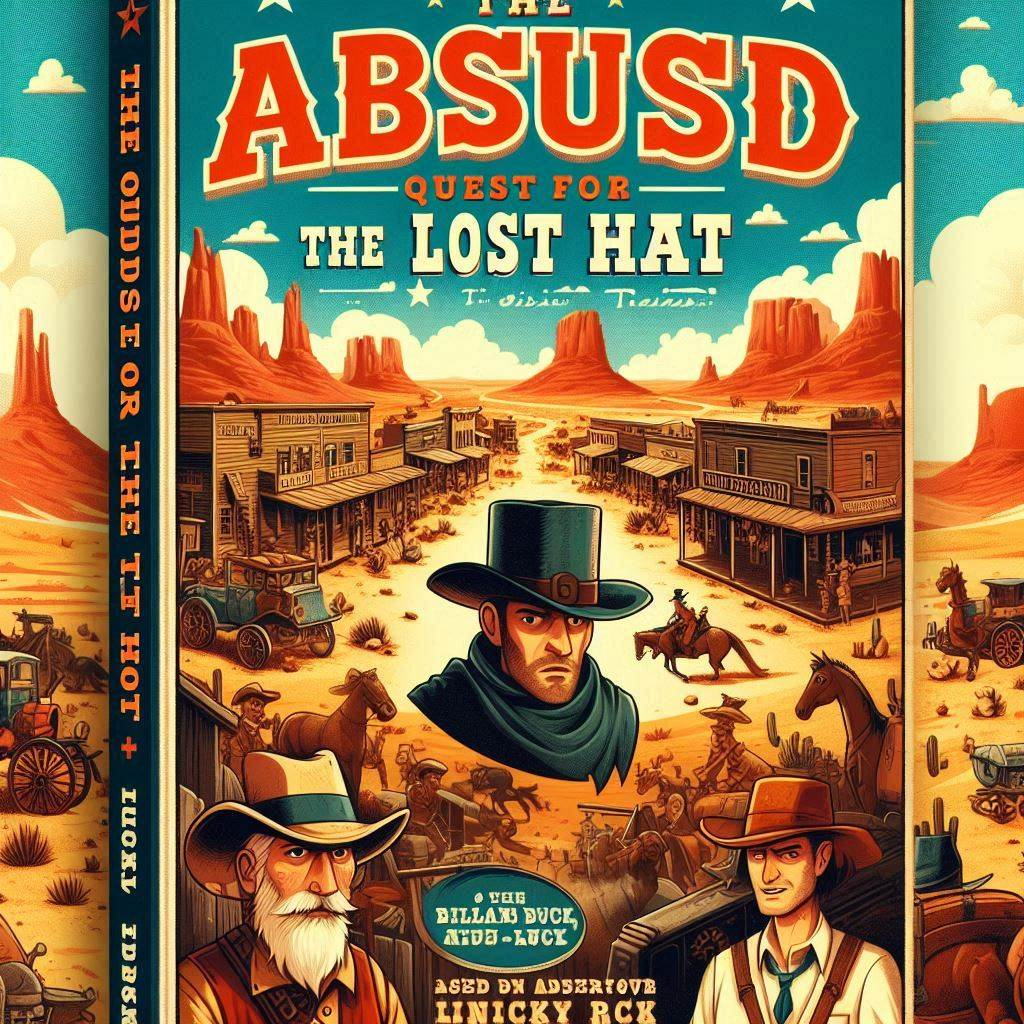
\includegraphics[width=0.9\textwidth]{ cover.jpg }
    \vfill
    \today
\end{titlepage}

\section*{Autorenvita}
\vspace{4cm}
Maja Schmidt ist eine bekannte und erfahrene Autorin von Fantasy-Büchern, die sich auf das Thema Studentenleben spezialisiert hat. Mit einer Leidenschaft für magische Welten und tiefgründige Charaktere hat sie bereits mehrere erfolgreiche Romane veröffentlicht. Ihre Geschichten zeichnen sich durch eine fesselnde Mischung aus Abenteuer, Selbstfindung und persönlicher Entwicklung aus.

\clearpage
\tableofcontents
\clearpage


\section{ Die Entdeckung der Magie }
Leon Weber betrat das weitläufige Gelände der Universität von Arcanum mit einem Gefühl der Aufregung und Nervosität. Die altehrwürdigen Gebäude und die lebhafte Atmosphäre ließen ihn sich klein und unbedeutend fühlen. Er hatte gerade sein Zimmer im Studentenwohnheim bezogen und war nun auf dem Weg zu seiner ersten Vorlesung. 

'Leon!' rief eine vertraute Stimme hinter ihm. Er drehte sich um und sah Mara Fischer, seine beste Freundin aus der Heimat, auf ihn zulaufen. 'Ich kann nicht glauben, dass wir es beide hierher geschafft haben!' 

'Ja, es ist wirklich unglaublich,' antwortete Leon und lächelte. 'Wie läuft es bei dir?' 

'Gut, ich habe gerade meine erste Vorlesung hinter mir. Es ist alles so aufregend und neu,' sagte Mara strahlend. 

Sie unterhielten sich noch eine Weile, bevor sie sich trennten, um zu ihren jeweiligen Vorlesungen zu gehen. Leon betrat den Hörsaal und setzte sich in eine der hinteren Reihen. Während der Professor über die Grundlagen der Physik sprach, konnte Leon seine Gedanken nicht von den seltsamen Ereignissen ablenken, die er in den letzten Tagen beobachtet hatte. 

Nach der Vorlesung beschloss er, den Campus zu erkunden. Er schlenderte durch die Gänge und bemerkte plötzlich ein Buch, das in der Luft schwebte. Er blinzelte und das Buch fiel zu Boden. Verwirrt hob er es auf und sah sich um, aber niemand schien es bemerkt zu haben. 

Später am Abend, als er in seinem Zimmer saß und über das seltsame Ereignis nachdachte, klopfte es an seiner Tür. Es war Professor Alaric Stern, ein älterer Mann mit durchdringenden Augen. 

'Herr Weber, ich habe gehört, dass Sie heute etwas Ungewöhnliches erlebt haben,' sagte der Professor. 

'Ja, ich... ich habe ein Buch gesehen, das in der Luft schwebte,' stotterte Leon. 

'Kommen Sie mit mir,' sagte Professor Stern und führte Leon durch eine verborgene Tür in der Bibliothek. 'Es gibt etwas, das Sie wissen müssen.' 

Leon folgte ihm und betrat eine geheime magische Bibliothek. 'Willkommen in der wahren Universität von Arcanum,' sagte Professor Stern. 'Hier werden Sie lernen, was es bedeutet, ein Magier zu sein.' Leon konnte kaum glauben, was er sah. Die geheime magische Bibliothek war riesig, mit Regalen, die bis zur Decke reichten und Bücher, die in der Luft schwebten. Professor Stern führte ihn zu einem Tisch, auf dem ein altes, verziertes Buch lag. 'Dies ist das Buch der Anfänge,' erklärte der Professor. 'Es enthält die Grundlagen der Magie, die jeder angehende Magier kennen muss.'

Leon öffnete das Buch vorsichtig und begann zu lesen. Die Worte schienen vor seinen Augen zu tanzen, und er spürte eine seltsame Energie durch seinen Körper fließen. 'Das ist unglaublich,' flüsterte er.

'Es wird noch unglaublicher,' sagte Professor Stern mit einem Lächeln. 'Aber zuerst müssen Sie die Grundlagen beherrschen. Ihre Ausbildung beginnt morgen früh.'

Am nächsten Tag traf Leon auf dem Hauptcampus auf Elena Schwarz, eine talentierte Studentin, die bereits von ihren Fähigkeiten bekannt war. 'Du bist der Neue, oder?' fragte sie neugierig.

'Ja, ich bin Leon,' antwortete er schüchtern.

'Ich bin Elena. Wenn du Hilfe brauchst, lass es mich wissen. Die ersten Tage können überwältigend sein,' sagte sie freundlich.

Leon nickte dankbar und machte sich auf den Weg zu seinem ersten magischen Unterricht. Der Raum war voller Studenten, die gespannt auf Professor Stern warteten. 'Heute werden wir die Grundlagen der Telekinese lernen,' begann der Professor. 'Konzentrieren Sie sich auf das Objekt vor Ihnen und versuchen Sie, es mit Ihrem Geist zu bewegen.'

Leon schloss die Augen und konzentrierte sich auf einen kleinen Stein vor ihm. Nach einigen Minuten spürte er, wie der Stein sich leicht hob. 'Ich habe es geschafft!' rief er begeistert.

'Gut gemacht, Herr Weber,' lobte Professor Stern. 'Aber das ist nur der Anfang. Es gibt noch viel zu lernen.'

Nach dem Unterricht traf Leon sich mit Mara, die neugierig auf seine neuen Erfahrungen war. 'Wie war dein Tag?' fragte sie.

'Es war unglaublich. Ich habe gelernt, wie man Dinge mit dem Geist bewegt,' erzählte Leon aufgeregt.

'Wow, das klingt fantastisch! Ich wünschte, ich könnte das auch sehen,' sagte Mara mit einem Lächeln.

'Vielleicht eines Tages,' antwortete Leon geheimnisvoll und dachte an die vielen Abenteuer, die noch vor ihm lagen. Leon fühlte sich überwältigt von den neuen Eindrücken und der Fülle an Informationen, die er in so kurzer Zeit aufgenommen hatte. Nach dem Unterricht machte er sich auf den Weg zur geheimen magischen Bibliothek, um weiter zu lernen. Dort traf er erneut auf Elena, die in einem alten Buch vertieft war.

'Hey Leon, wie läuft es bei dir?' fragte sie, ohne den Blick von den Seiten zu heben.

'Es ist unglaublich, aber auch ziemlich viel auf einmal,' antwortete Leon ehrlich. 'Ich habe das Gefühl, dass ich noch so viel lernen muss.'

Elena lächelte und klappte ihr Buch zu. 'Das geht uns allen so. Aber du wirst sehen, mit der Zeit wird es einfacher. Wenn du möchtest, können wir zusammen lernen. Zwei Köpfe sind besser als einer.'

'Das wäre großartig, danke,' sagte Leon erleichtert.

In den nächsten Tagen verbrachten Leon und Elena viel Zeit zusammen, sowohl im Unterricht als auch in der Bibliothek. Sie half ihm, die komplexen magischen Konzepte zu verstehen, und er begann, sich sicherer zu fühlen. Professor Stern beobachtete ihre Fortschritte mit Wohlwollen.

Eines Abends, als Leon sich auf den Weg zurück ins Studentenwohnheim machte, traf er auf Mara, die auf ihn wartete. 'Hey, wie war dein Tag?' fragte sie neugierig.

'Es war gut. Ich habe viel gelernt und Elena hat mir wirklich geholfen,' erzählte Leon.

'Ich bin froh, dass du Freunde gefunden hast. Aber vergiss nicht, auch mal eine Pause zu machen,' riet Mara mit einem Lächeln.

'Keine Sorge, ich werde schon auf mich aufpassen,' versicherte Leon ihr.

Die Tage vergingen und Leon wurde immer vertrauter mit der magischen Welt. Er meisterte die Grundlagen der Telekinese und begann, sich auch in anderen magischen Disziplinen zu üben. Professor Stern war beeindruckt von Leons Fortschritten und ermutigte ihn, weiterzumachen.

Eines Nachmittags, als Leon und Elena in der Bibliothek studierten, kam Professor Stern auf sie zu. 'Herr Weber, Fräulein Schwarz, ich möchte Ihnen beiden für Ihre harte Arbeit danken. Sie machen große Fortschritte. Aber denken Sie daran, dies ist erst der Anfang. Es gibt noch viel zu lernen und zu entdecken.'

'Wir werden unser Bestes geben, Professor,' antwortete Elena entschlossen.

Leon nickte zustimmend. 'Ja, wir sind bereit für die nächsten Herausforderungen.'

Mit diesen Worten fühlte Leon eine neue Welle der Entschlossenheit in sich aufsteigen. Er wusste, dass er auf dem richtigen Weg war und dass die magische Welt noch viele Geheimnisse für ihn bereithielt.

\section{ Ein Jahr im Verborgenen }
Leon hatte sich mittlerweile gut in die magische Gemeinschaft integriert. Er und Elena verbrachten fast jede freie Minute zusammen, sei es im Unterricht, in der Bibliothek oder bei Spaziergängen durch den magischen Wald. Ihre Freundschaft wuchs stetig, und sie lernten viel voneinander.

Eines Nachmittags saßen sie in der Bibliothek, als Elena plötzlich fragte: 'Leon, hast du schon mal darüber nachgedacht, wie dein Leben ohne die Magie wäre?'

Leon legte sein Buch zur Seite und dachte nach. 'Ehrlich gesagt, nein. Seit ich hier bin, fühlt es sich an, als hätte ich endlich meinen Platz gefunden. Aber manchmal frage ich mich, wie es Mara geht. Sie weiß nichts von all dem hier.'

Elena nickte verständnisvoll. 'Es muss schwer sein, ein Doppelleben zu führen. Aber du machst das großartig. Und Mara scheint eine tolle Freundin zu sein.'

'Ja, das ist sie,' sagte Leon lächelnd. 'Sie unterstützt mich, auch wenn sie nicht alles versteht.'

In diesem Moment betrat Professor Stern die Bibliothek. 'Herr Weber, Fräulein Schwarz, ich sehe, Sie arbeiten fleißig. Wie laufen Ihre Studien?'

'Gut, Professor,' antwortete Elena. 'Wir machen Fortschritte.'

'Freut mich zu hören,' sagte Professor Stern. 'Denken Sie daran, dass es wichtig ist, ein Gleichgewicht zu finden. Die magische Welt ist faszinierend, aber vergessen Sie nicht, auch Ihre anderen Verpflichtungen zu erfüllen.'

Leon nickte. 'Ja, Professor. Ich werde daran denken.'

Später an diesem Abend traf Leon sich mit Mara in einem Café in der Stadt. 'Wie läuft es an der Uni?' fragte sie neugierig.

'Es ist viel zu tun, aber ich komme zurecht,' antwortete Leon. 'Und ich habe tolle Freunde gefunden, die mir helfen.'

'Ich bin froh, das zu hören,' sagte Mara lächelnd. 'Vergiss nicht, auch mal abzuschalten und Spaß zu haben.'

'Keine Sorge, das werde ich,' versicherte Leon ihr.

Die Tage vergingen, und Leon fand immer besser seinen Platz in beiden Welten. Er lernte, seine Zeit zu managen und die Balance zwischen seinem normalen und magischen Leben zu halten. Mit der Unterstützung von Elena, Professor Stern und Mara fühlte er sich bereit für die kommenden Herausforderungen. Leon kämpfte zunehmend mit den Anforderungen seines Doppellebens. Die magischen Studien wurden intensiver, und die Prüfungen an der Universität von Arcanum forderten ihn heraus. Gleichzeitig musste er seine Verpflichtungen in der normalen Welt erfüllen, was ihn oft an seine Grenzen brachte.

Eines Abends, nach einem besonders anstrengenden Tag, saß Leon erschöpft in seinem Zimmer im Studentenwohnheim. Ein Klopfen an der Tür riss ihn aus seinen Gedanken. Es war Elena.

'Leon, alles in Ordnung?' fragte sie besorgt.

'Es ist nur... alles wird mir gerade zu viel,' gestand Leon. 'Die Prüfungen, die Geheimhaltung, das ständige Hin und Her. Ich weiß nicht, wie lange ich das noch durchhalte.'

Elena setzte sich neben ihn. 'Ich verstehe, wie du dich fühlst. Aber du bist nicht allein. Wir sind alle hier, um dir zu helfen. Und vergiss nicht, was Professor Stern gesagt hat: Es ist wichtig, ein Gleichgewicht zu finden.'

Leon nickte langsam. 'Du hast recht. Ich muss einen Weg finden, besser mit allem umzugehen.'

Am nächsten Tag suchte Leon das Gespräch mit Professor Stern. 'Professor, ich brauche Ihre Hilfe. Ich habe Schwierigkeiten, mein Doppelleben zu managen.'

Professor Stern sah ihn aufmerksam an. 'Das ist verständlich, Leon. Viele junge Magier haben ähnliche Probleme. Es erfordert Disziplin und Organisation. Aber vor allem musst du lernen, dir selbst Pausen zu gönnen und Prioritäten zu setzen.'

'Danke, Professor. Ich werde es versuchen,' sagte Leon entschlossen.

Später traf er sich mit Mara, die sofort bemerkte, dass etwas nicht stimmte. 'Leon, du siehst erschöpft aus. Was ist los?'

'Es ist nur der ganze Stress,' antwortete Leon. 'Aber ich arbeite daran, besser damit umzugehen.'

Mara lächelte aufmunternd. 'Du schaffst das. Und wenn du mal reden musst, bin ich immer für dich da.'

Mit der Unterstützung von Elena, Professor Stern und Mara begann Leon, seine Zeit besser zu managen. Er setzte sich klare Ziele und nahm sich bewusst Auszeiten, um sich zu erholen. Langsam aber sicher fand er eine Balance zwischen seinen beiden Welten und fühlte sich gestärkt für die kommenden Herausforderungen. Das Semester neigte sich dem Ende zu, und die Prüfungen standen bevor. Leon hatte hart gearbeitet, um seine Balance zu finden, doch die bevorstehenden Herausforderungen ließen ihn nicht zur Ruhe kommen. Eines Abends, als er in der geheimen magischen Bibliothek studierte, kam Elena aufgeregt auf ihn zu.

'Leon, hast du schon von der großen Prüfung gehört?' fragte sie atemlos.

'Welche Prüfung?' erwiderte Leon verwirrt.

'Die Prüfung der Elemente. Jeder Student muss sie bestehen, um ins nächste Jahr aufzusteigen. Es ist eine der härtesten Prüfungen an der Universität von Arcanum.'

Leon schluckte. 'Ich habe davon gehört, aber ich dachte, sie wäre nur ein Gerücht.'

'Nein, sie ist real. Und wir müssen uns darauf vorbereiten,' sagte Elena entschlossen.

Die nächsten Tage verbrachten Leon und Elena damit, sich intensiv auf die Prüfung vorzubereiten. Professor Stern unterstützte sie mit zusätzlichen Lektionen und wertvollen Ratschlägen.

'Am wichtigsten ist es, ruhig zu bleiben und sich auf das zu konzentrieren, was ihr gelernt habt,' sagte Professor Stern. 'Vertraut auf eure Fähigkeiten.'

Am Tag der Prüfung versammelten sich die Studenten im magischen Wald. Die Atmosphäre war angespannt. Leon spürte, wie sein Herz schneller schlug, als er an der Reihe war. Die Prüfung begann mit einer Reihe von Aufgaben, die seine Kontrolle über die Elemente testeten.

Er musste Feuer entfachen, Wasser bändigen, die Erde formen und den Wind lenken. Jede Aufgabe war eine Herausforderung, doch Leon erinnerte sich an die Worte von Professor Stern und blieb konzentriert. Mit jeder bestandenen Aufgabe wuchs sein Selbstvertrauen.

Als die Prüfung vorbei war, fühlte sich Leon erschöpft, aber auch erleichtert. Er hatte es geschafft. Elena kam auf ihn zu und umarmte ihn.

'Wir haben es geschafft, Leon!'

'Ja, das haben wir,' sagte Leon lächelnd.

Später traf er sich mit Mara, um ihr von der Prüfung zu erzählen. 'Es war unglaublich anstrengend, aber ich habe es geschafft,' sagte er stolz.

'Ich wusste, dass du es schaffst,' sagte Mara und umarmte ihn. 'Du bist stärker, als du denkst.'

Mit der Unterstützung seiner Freunde und Mentoren hatte Leon eine bedeutende Hürde überwunden. Er fühlte sich bereit für die kommenden Herausforderungen und war gespannt, was das nächste Jahr an der Universität von Arcanum für ihn bereithalten würde.

\clearpage

\section*{Metadaten}
\colorbox{lightgray}{
    \begin{minipage}{\dimexpr\textwidth-2\fboxsep}
        \vspace{1cm}
        \begin{itemize}
            \item Name des Buches: Die Magische Universität: Ein Jahr im Verborgenen
            \item Name des Autors: Maja Schmidt
            \item Name des Herausgebers: Mark Zimmermann
            \item Name des Verlags: HdM AI Technologies
            \item Adresse des Verlags: Nobelstraße 10, 70569 Stuttgart
            \item Datum der Veröffentlichung: 2023-10-10
        \end{itemize}
        \vspace{1cm}
    \end{minipage}
}

\end{document}